\section{Experiments}
\label{sec:experiments}

We now return to the original question of the paper: is planning technology
ready for realistic applications in natural language generation? To investigate
this question we consider two sets of experiments, designed to evaluate the
performance of several planners on the NLG planning domains from the previous
section. Starting with the CRISP domain, we first present a scenario which
focuses on the generation of referring expressions with a tiny grammar
(Section~\ref{sec:exper-1:-sent}). We then look at a setting in which CRISP is
used for surface realization with the XTAG Grammar \citep{xtag01:_tr}, a
large-scale TAG grammar for English (Section~\ref{sec:exper-2:-sent-xtag}). In
the second set of experiments we investigate the GIVE domain. We begin with a
domain that is similar to the classic Gridworld
(Section~\ref{sec:exper-3:-minim}), and then add extra grid cells to the world
that are not necessary to complete the task
(Section~\ref{sec:experiment-4:-give}). We also investigate the role that goal
ordering plays in these problems. These experiments are configured in a way that
lets us explore the scalability of a planner's search and preprocessing
capabilities, and illustrates what we perceive to be one of the main limitations
of current off-the-shelf planners for our applications: they often spend a long
time computing ground instances, even when most of these instances are not
required during plan search.



\subsection{Experiment 1: Sentence generation (referring expressions)}
\label{sec:exper-1:-sent}

For the first experiment on sentence generation, we exercise the
ability of the CRISP system described in
Section~\ref{sec:domain-crisp} to generate referring expressions. This
problem is usually handled by the sentence planner if sentence
planning and surface realization are separated; here it happens as
part of the overall generation process. 

We consider a series of sentence generation problems which require the
planner to compute a plan representing the sentence ``Mary likes the
Adj$_1$ \ldots Adj$_n$ rabbit.''  Each problem instance assumes a
target referent $r$, which is a rabbit, and a certain number $m$ of
further rabbits $r_1,\ldots,r_m$ that are distinguished by properties
$P_1,\ldots,P_n$ with $n \leq m$. The problem instance is set up such
that $r$ has all properties except for $P_i$ in common with each $r_i$
for $1 \leq i \leq n$, and $r_{n+1},\ldots,r_m$ have none of the
properties $P_i$. That is, all $n$ properties are required to describe
$r$ uniquely. The $n$ properties are realized as $n$ different
adjectives, in any order.  This setup allows us to vary the plan
length (a plan with $n$ properties will have length $n+4$) and the
universe size (the universe will contain $m+1$ rabbit individuals in
addition to the individuals used to encode the grammar, which have
different types).

\begin{figure}
  \centering
  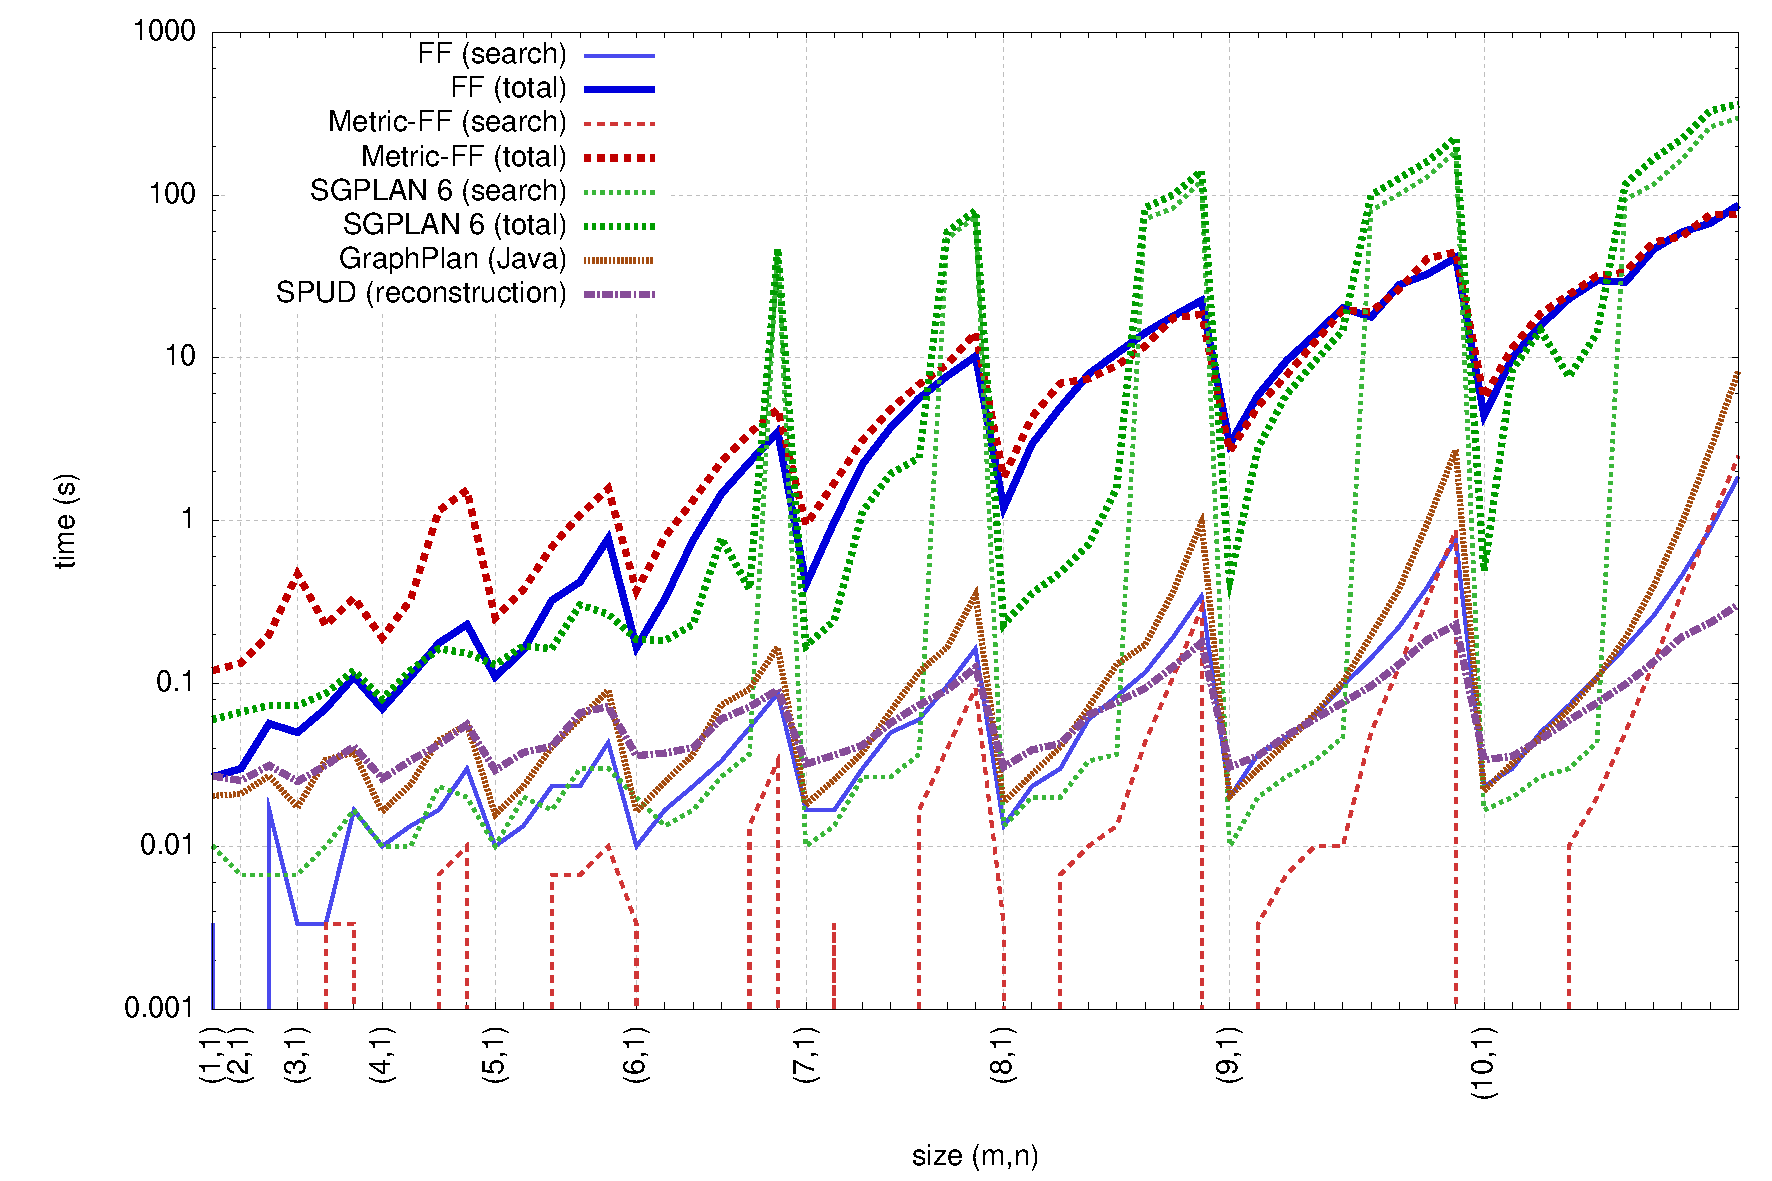
\includegraphics[width=\columnwidth]{data/modifiers-all}
  \caption{Results for the sentence generation domain. The
    horizontal axis represents parameters $(m,n)$ from $(1,1)$ to
    $(10,10)$ in lexicographical order. The vertical axis is the
    runtime in milliseconds.}
  \label{fig:runtimes-crisp}
\end{figure}

We converted these generation problem instances into planning problem
instances as described in Section~\ref{sec:domains}, and then ran
several different planners on them. We used three off-the-shelf
planners: FF 2.3 \citep{HoffmannNebel01}, Metric-FF
\citep{hoffmann:ecai-02}, and SGPLAN 6
\citep{hsu06:_new_featur_in_sgplan_for}; all of these were highly
successful at the recent IPC competitions, and unlike many other IPC
participants, support a fragment of PDDL with quantified and
conditional effects, which is necessary in our domain. In addition, we
used an ad-hoc implementation of GraphPlan \citep{Blum1997} written in
Java; unlike the three off-the-shelf planners, it only computes
instances of literals and operators as they are needed in the course
of the plan search, instead of computing all ground instances in a
separate preprocessing step. Finally, we reimplemented the incomplete
greedy search algorithm used in the SPUD system \citep{Stone2003a} in
Java.

The results of this experiment are shown in the graph in
Figure~\ref{fig:runtimes-crisp}.\footnote{All runtimes in
  Sections~\ref{sec:exper-1:-sent} and \ref{sec:exper-2:-sent-xtag}
  were measured on a single core of an AMD Opteron 8220 CPU running at
  2.8 GHz, under Linux. FF 2.3 and Metric-FF were recompiled as 64-bit
  binaries and run with a memory limit of 32 GB. Java programs were
  executed under Java 1.6.0\_13 in 64-bit mode and were allowed to
  ``warm up'', i.e., the JVM was given the opportunity to just-in-time
  compile the relevant bytecode by running the planner three times and
  discarding the runtimes before taking the actual measurements. All
  runtimes are averaged over three runs of the planners.} The input
parameters $(m,n)$ are plotted in lexicographic order on the
horizontal axis, and the runtime is shown in seconds on the vertical
axis, on a logarithmic scale. These results reveal a number of
interesting insights. First, the search times of FF and Metric-FF
(shown as thinner lines) significantly outperform SGPLAN's search in
this domain---on the largest instances, by a factor of over
100.\footnote{For FF and Metric-FF, we report the ``searching'' and
  ``total'' times reported by the planners. For SGPLAN, we report the
  ``total'' time and the difference between the ``total'' and
  ``parsing'' times.} Second, FF and Metric-FF perform very similarly
to each other, and their search times are almost the same as those of
the SPUD algorithm, which is impressive because they are complete
search algorithms, whereas SPUD's greedy algorithm is not.

Finally, it is striking that for all three off-the-shelf planners, the
search only accounts for a tiny fraction of the total runtime; in each
case, the preprocessing times are higher than the search times by one
or two orders of magnitude. As a consequence, even our relatively
naive Java implementation of GraphPlan outperforms them all in terms
of total runtime, because it only computes instances by need. Although
FF is consistently much faster as far as pure search time is
concerned, our results indicate that FF's performance is much more
sensitive to the domain size: if we fix $n=1$, FF takes 27
milliseconds to compute a plan at $m=1$, but 4.4 seconds to compute
the same plan at $m=10$. By comparison, our GraphPlan implementation
takes 20 ms at $m=1$ and still only requires 22 ms at
$m=10$.



\subsection{Experiment 2: Sentence generation (XTAG)}
\label{sec:exper-2:-sent-xtag}

The first experiment already gives us some initial insights into the
appropriateness of planning for the sentence generation domain: On the
examples we looked at, the search times were quite acceptable, but FF
and SGPLAN spent a lot of time on the initial grounding step.
However, one weakness of this experiment is that it uses a tiny
grammar, consisting of just those 12 lexicon entries that are needed
for the experiment. While the grounding problem can only get worse
with larger grammars, the experiment by itself does not allow us to
make clear statements about the search efficiency.
To address this problem, we ran a second sentence generation
experiment. This time, we used the XTAG Grammar \citep{xtag01:_tr}, a
large-scale TAG grammar of English. XTAG contains lexicon entries for
about 17,000 uninflected words using about 1100 different elementary
trees. Although XTAG does not contain semantic information, it is
possible to automatically equip the lexicon entries with inferred
semantic representations based on the words in the lexicalized
elementary trees. The result is a highly ambiguous grammar: The most
ambiguous word, ``ask'', is the anchor of 314 lexicon entries.

In our experiment, we were especially interested in two
questions. First, how would the planners handle the search problem
involved in generating with such a large and ambiguous grammar?
Second, would it be harder to generate sentences containing verbs with
multiple arguments, given that verbs with more arguments lead to
actions with more parameters and therefore more instances? To answer
these questions, we generated sentences of the form ``S and S and
\ldots and S'', where each S was a sentence; we called the number of
sentences in the conjunction $n$. Each S was a sentence of the form
``the businessman sneezes'', ``the businessman admires the girl'', or
``the businessman gives the girl the book''---that is, they varied in
the number $k$ of syntactic arguments the verb expects (1 for the
intransitive verb ``sneeze'', 2 for the transitive verb ``admire'',
and 3 for the ditransitive verb ``give''). This means that the output
sentence for parameters $n$ and $k$ contained $n(2k+2)-1$ words. The
instances were set up in such a way that the generation of referring
expressions was trivial, so this experiment was purely a surface
realization task. To achieve reasonable performance, we only generated
planning operators for those elementary trees for which all predicate
symbols in the semantic representation also appeared in the knowledge
base.

\begin{figure}[t]
\subfloat[$k=1$]{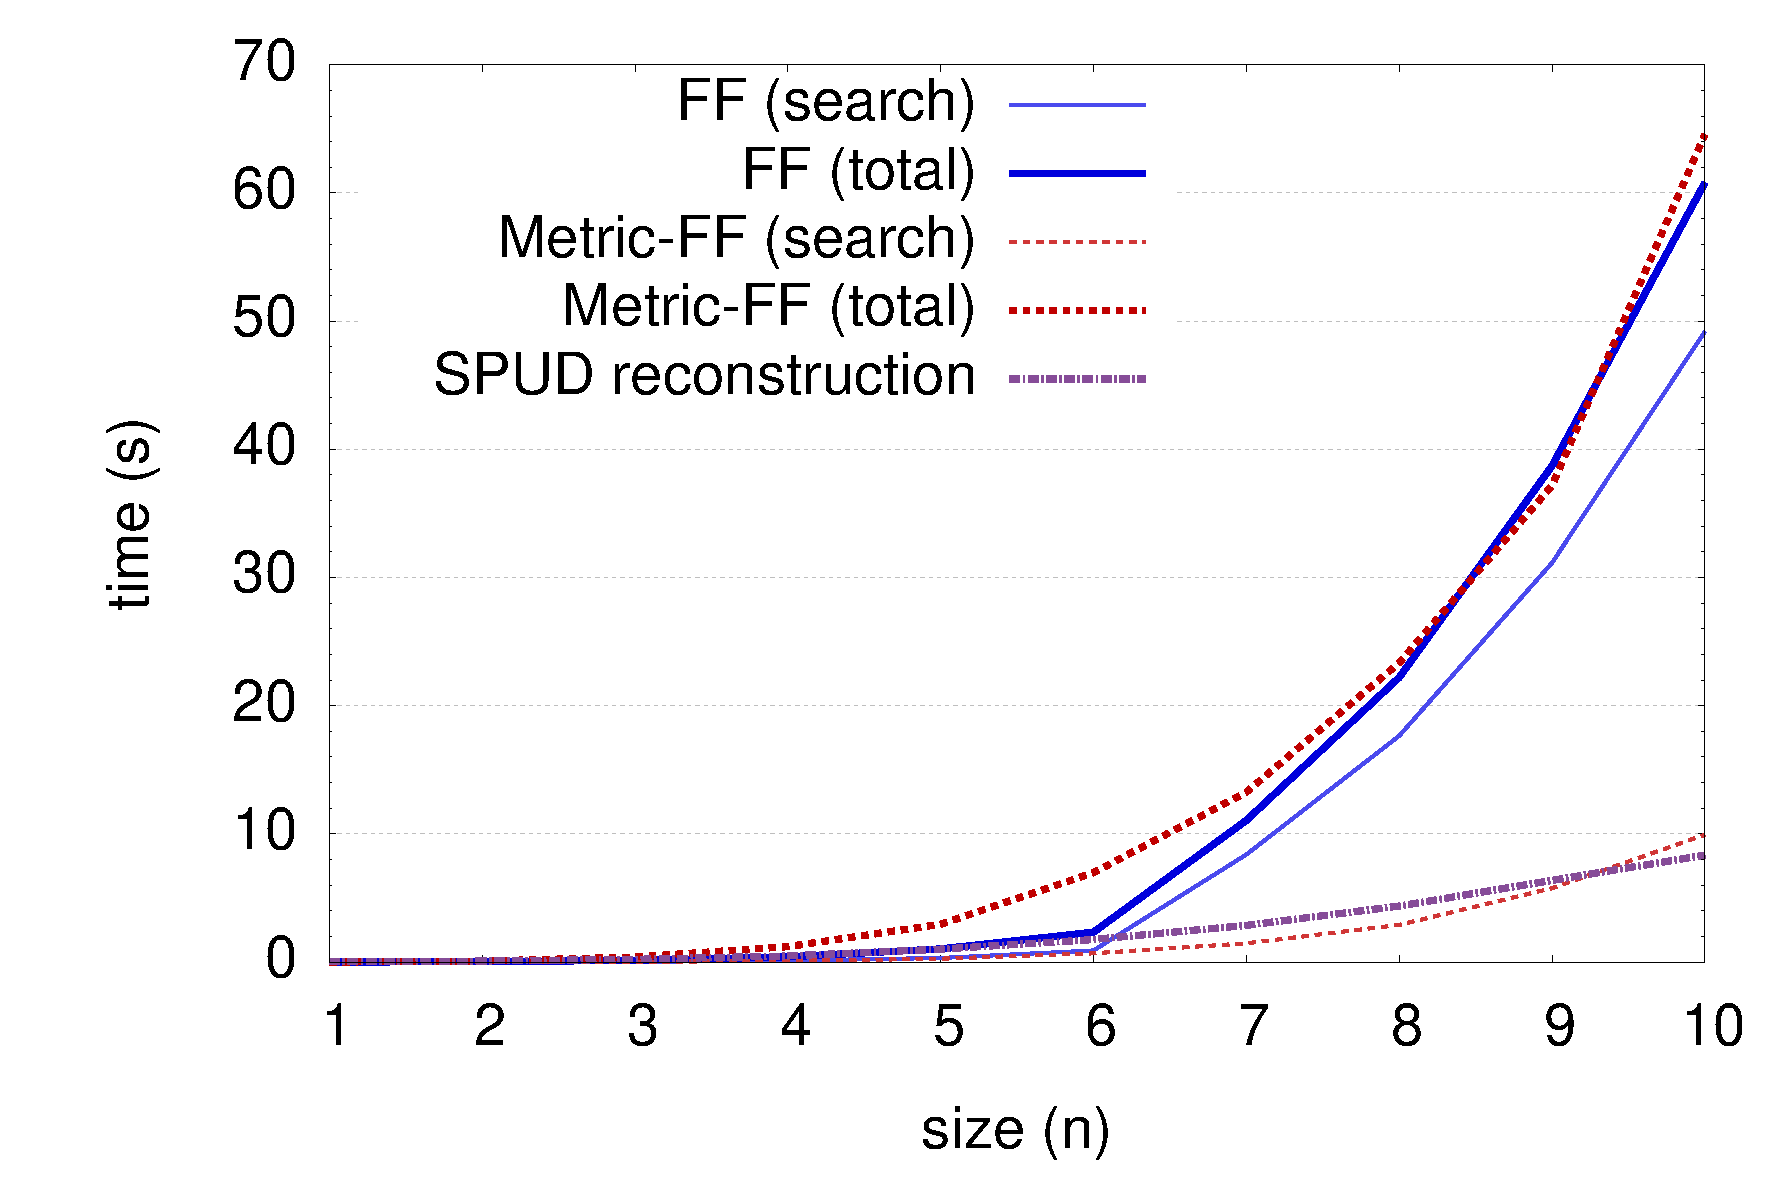
\includegraphics[width=7cm]{data/xtag-k1.pdf}}
\subfloat[$k=2$]{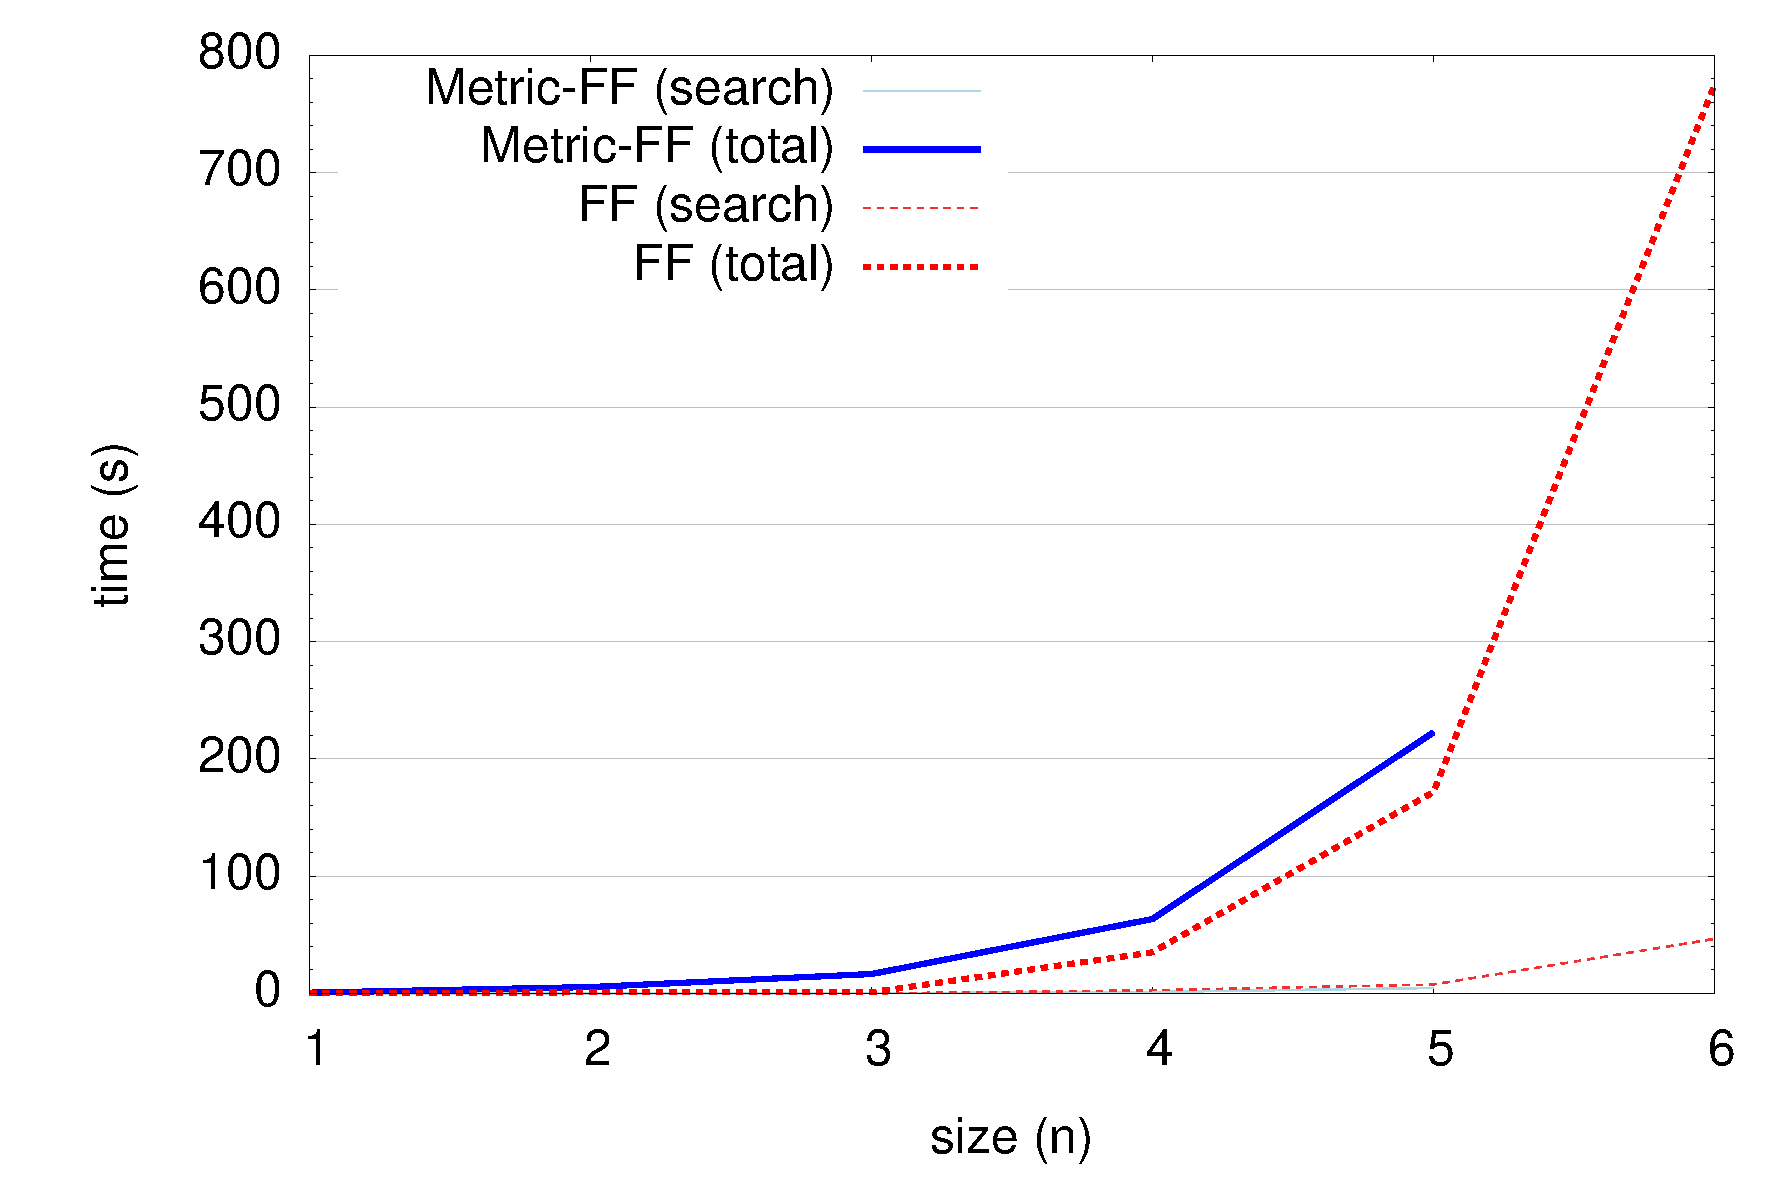
\includegraphics[width=7cm]{data/xtag-k2.pdf}}
  \caption{Results for the XTAG experiment, at $k=1$ and $k=2$.}
  \label{fig:xtag-graph}
\end{figure}

Fig.~\ref{fig:xtag-graph} reports the runtimes we measured in this
experiment for FF, Metric FF, and the SPUD reimplementation. We do not
report runtimes for SGPLAN, because we could not recompile SGPLAN as a
64-bit binary, and the 32-bit version ran out of memory very
quickly. We also do not report runtimes for our Java implementation of
Graphplan, because it was unusuably slow for serious problem
instances: For $k=1$ and $n=3$, it already took over two minutes, and
it exceeded its memory limit of 16 GB for $n>3$. This may be a
limitation of our naive implementation rather than the GraphPlan
algorithm itself.

Nonetheless, there are a number of observations we can make in this
experiment. First of all, the experiment confirms that FF's Enforced
Hill-Climbing search strategy works very well for the sentence
generation task: Although we are now generating with a large grammar,
FF generates a 39-word sentence ($k=1,n=6$) in under a second of
search time. This level of efficiency is a direct result of using this
particular search strategy: For $k=1$ and $n>6$, FF 2.3 (but not
Metric-FF) fell back to the best-first search strategy, which causes a
dramatic loss of search effiency. It is also encouraging that
Metric-FF still performs comparably to SPUD in terms of pure search
time. We believe that by FF's technique of evaluating actions by
estimating the distance to a goal state for the relaxed problem
essentially picks out the same evaluation function as SPUD's domain-specific
heuristic, and the enforced hill-climbing strategy needs to backtrack
very little in this domain and thus performs similarly to SPUD's
greedy search. However, SPUD's incompleteness manifests itself in this
experiment by its inability to find any plan for $k>1$ and $n>1$,
whereas FF and its variants still (correctly) find these plans.

Second, FF's runtime is still dominated by the preprocessing
stage. For instance, Metric-FF spends about 10 seconds on search for
$k=1,n=10$, compared to its total runtime of about 65 seconds. This
effect becomes more pronounced as we increase $k$: For $k=2$, we reach
65 seconds of total runtime at $n=4$, but here Metric-FF only spends
about a second on search. For $k=3$, neither FF nor Metric-FF were
able to solve any of the input instances within their memory
limit. This is consistent with the observation that the planning
operators for the verbs have $k+2$ parameters (see
Fig.~\ref{fig:white-rabbit-as-planning}), and thus the number of
action instances grows by a factor of the universe size every time we
increase $k$ by one. A planner which computes all ground instances of
the operators thus takes exponential time in $k$ for preprocessing.

\begin{figure}[t]
  \centering
  \subfloat[position=bottom][(a) Minimal GIVE world]{%
      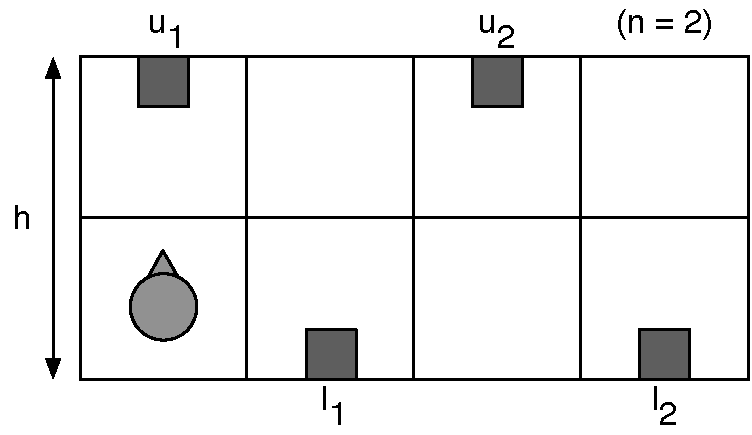
\includegraphics[height=2.5cm,clip=true,trim=0 -10px 0 -3px]{pic-buttons}}
  \qquad
  \subfloat[position=bottom][(b) GIVE world with extra grid cells]{%
      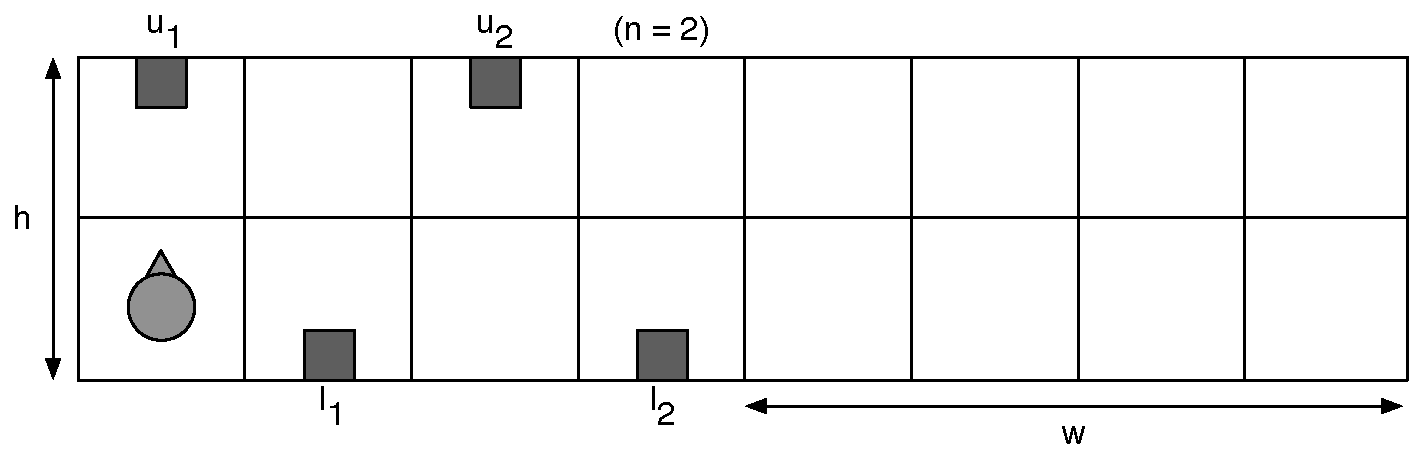
\includegraphics[height=2.5cm]{pic-empty-buttons}} \\
  %\subfloat[(c) Extra grid cells with inaccessible positions]{%
  %    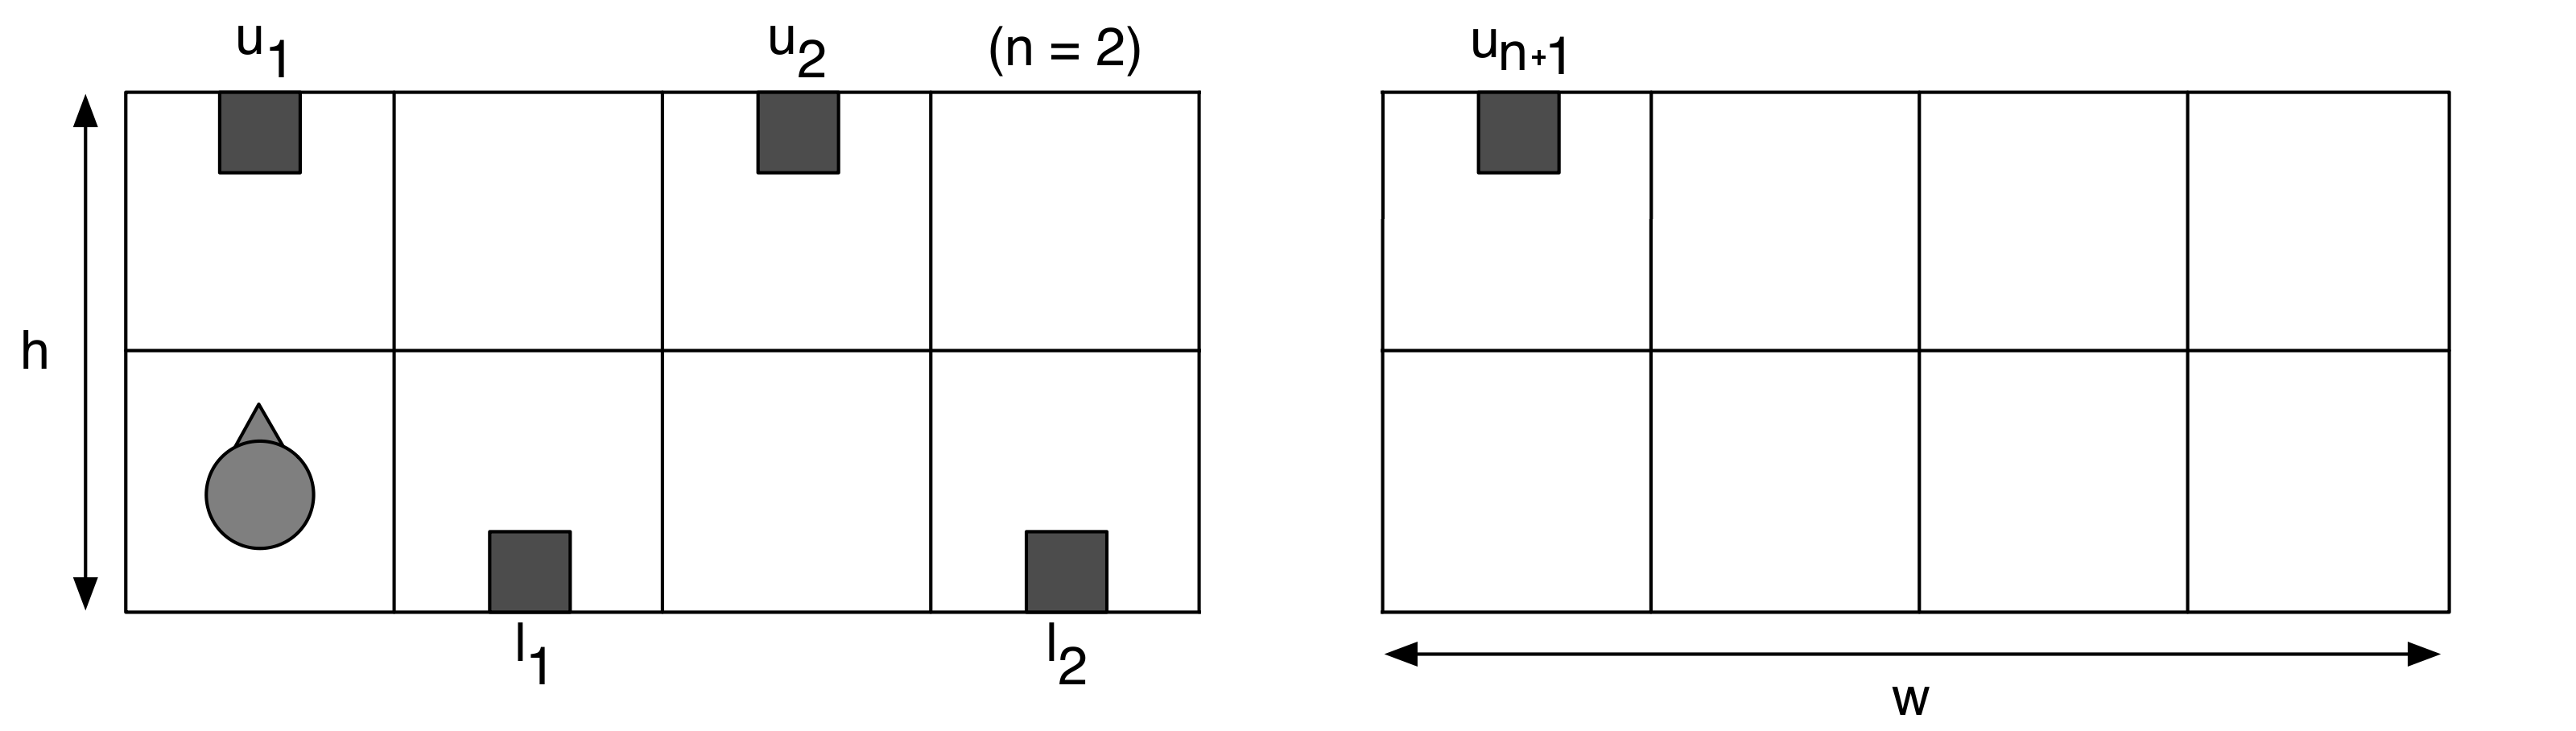
\includegraphics[height=2.5cm]{pic-empty-inaccessible}}
  \caption{Experimental GIVE world configurations.}
  \label{fig:give-maps}
\end{figure}


\subsection{Experiment 3: Minimal GIVE worlds}
\label{sec:exper-3:-minim}

We now turn our attention to a set of experiments arising from the GIVE domain.
Besides using many of the planners from the previous set of experiments (FF,
Metric-FF, and SGPLAN), we also expand our testing to include the FF(h$_a$)
\citep{keyder08:_ff_h_plann_for_plann}, LAMA \citep{richter08:_lama_plann}, and
C$^3$ \citep{lipovetzky08:_c3} planners. Each of these additional planners
competed in the deterministic ``sequential, satifying'' track of the 2008
International Planning Competition; all planners performed well on the
competition domains, with LAMA the overall winner of the track.\footnote{See
\texttt{http://ipc.informatik.uni-freiburg.de/} for details of the 2008 IPC.}

In the first GIVE experiment, we construct a series of grid worlds, similar to
the one illustrated in Figure~\ref{fig:give-maps}(a). These worlds consist of a
$N = 2n$ by $h$ grid of positions, such that there are buttons at positions
$(2i-1,1)$ and $(2i,h)$ for $1 \leq i \leq n$. The player starts in position
$(1,1)$ and must press all the buttons to successfully complete the game.  (The
actions in this domain are similar to the PDDL actions in
Figure~\ref{fig:give-planning}.) We consider two variants of this problem in our
tests. In the \emph{unordered} problem, the player is permitted to press the
buttons in any order to successfully achieve the goal. In the \emph{ordered}
version of the problem, the player is unable to initially move to any grid cell
containing a button, except for the cell containing the first button, $u_1$.
Pressing $u_1$ releases the position of the next button, $l_1$, allowing the
player to move into this cell.  Similarly, pressing button $l_1$ frees button
$u_2$, and so on. The end result is a set of constraints that forces the buttons
to be pressed in a particular order to achieve the goal. As a concrete example,
the following is a minimal plan (in either variant of the problem) for the case
of a $2$ by $2$ grid with $2$ buttons (i.e., $n=1$, $h=2$):

\begin{enumerate}
\item $\mathsf{move}(\mathsf{pos\_1\_1},\mathsf{pos\_1\_2}, \mathsf{north})$,
\item $\mathsf{manipulate}\textsf{-}\mathsf{button}\textsf{-}\mathsf{off}\textsf{-}\mathsf{on}(\mathsf{u1, pos\_1\_2})$,
\item $\mathsf{turn}\textsf{-}\mathsf{right}(\mathsf{north}, \mathsf{east})$,
\item $\mathsf{move}(\mathsf{pos\_1\_2}, \mathsf{pos\_2\_2},
  \mathsf{east})$,
\item $\mathsf{turn}\textsf{-}\mathsf{right}(\mathsf{east}, \mathsf{south})$,
\item $\mathsf{move}(\mathsf{pos\_2\_2}, \mathsf{pos\_2\_1}, \mathsf{south})$,
\item $\mathsf{manipulate}\textsf{-}\mathsf{button}\textsf{-}\mathsf{off}\textsf{-}\mathsf{on}(\mathsf{l1, pos\_2\_1})$.
\end{enumerate}

\begin{figure}[t]
\subfloat[(a) Unordered]{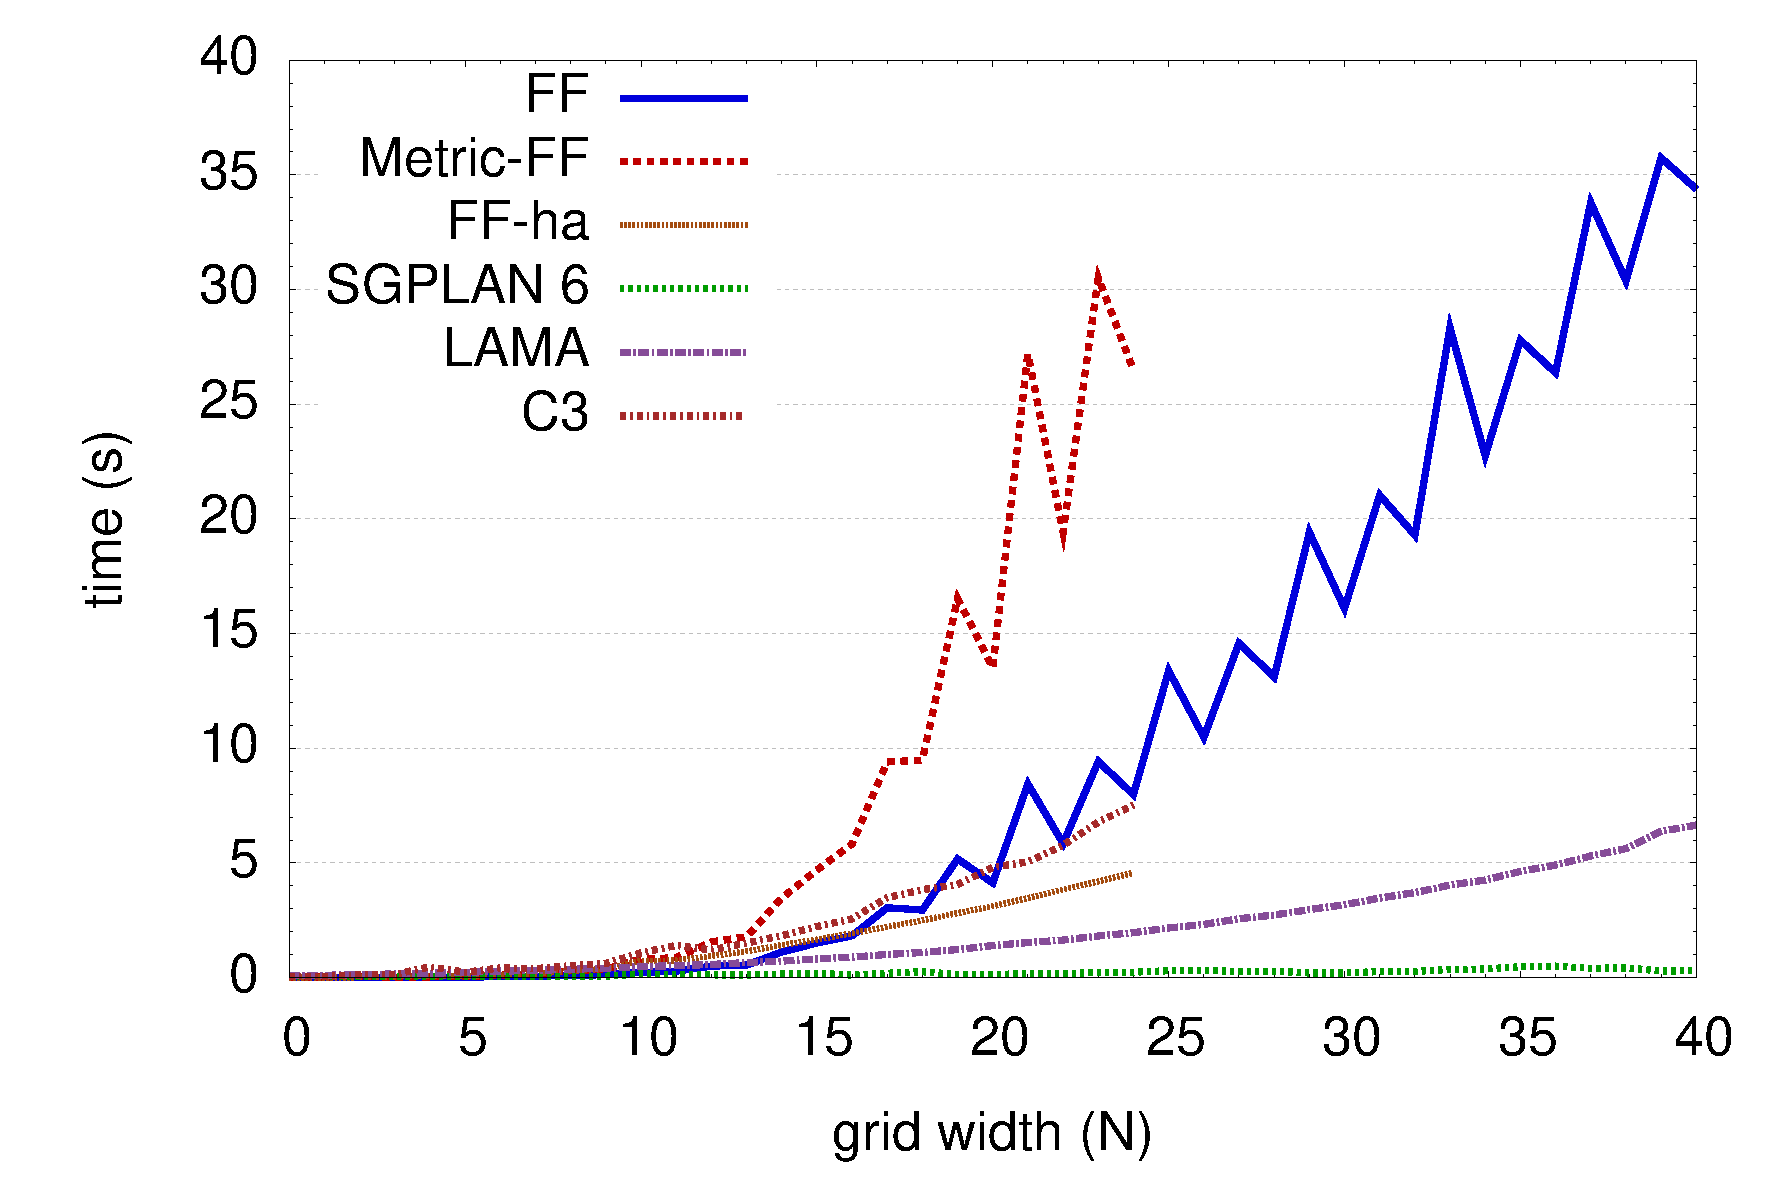
\includegraphics[width=7cm]{data/give-minimal.pdf}}
\subfloat[(b) Ordered]{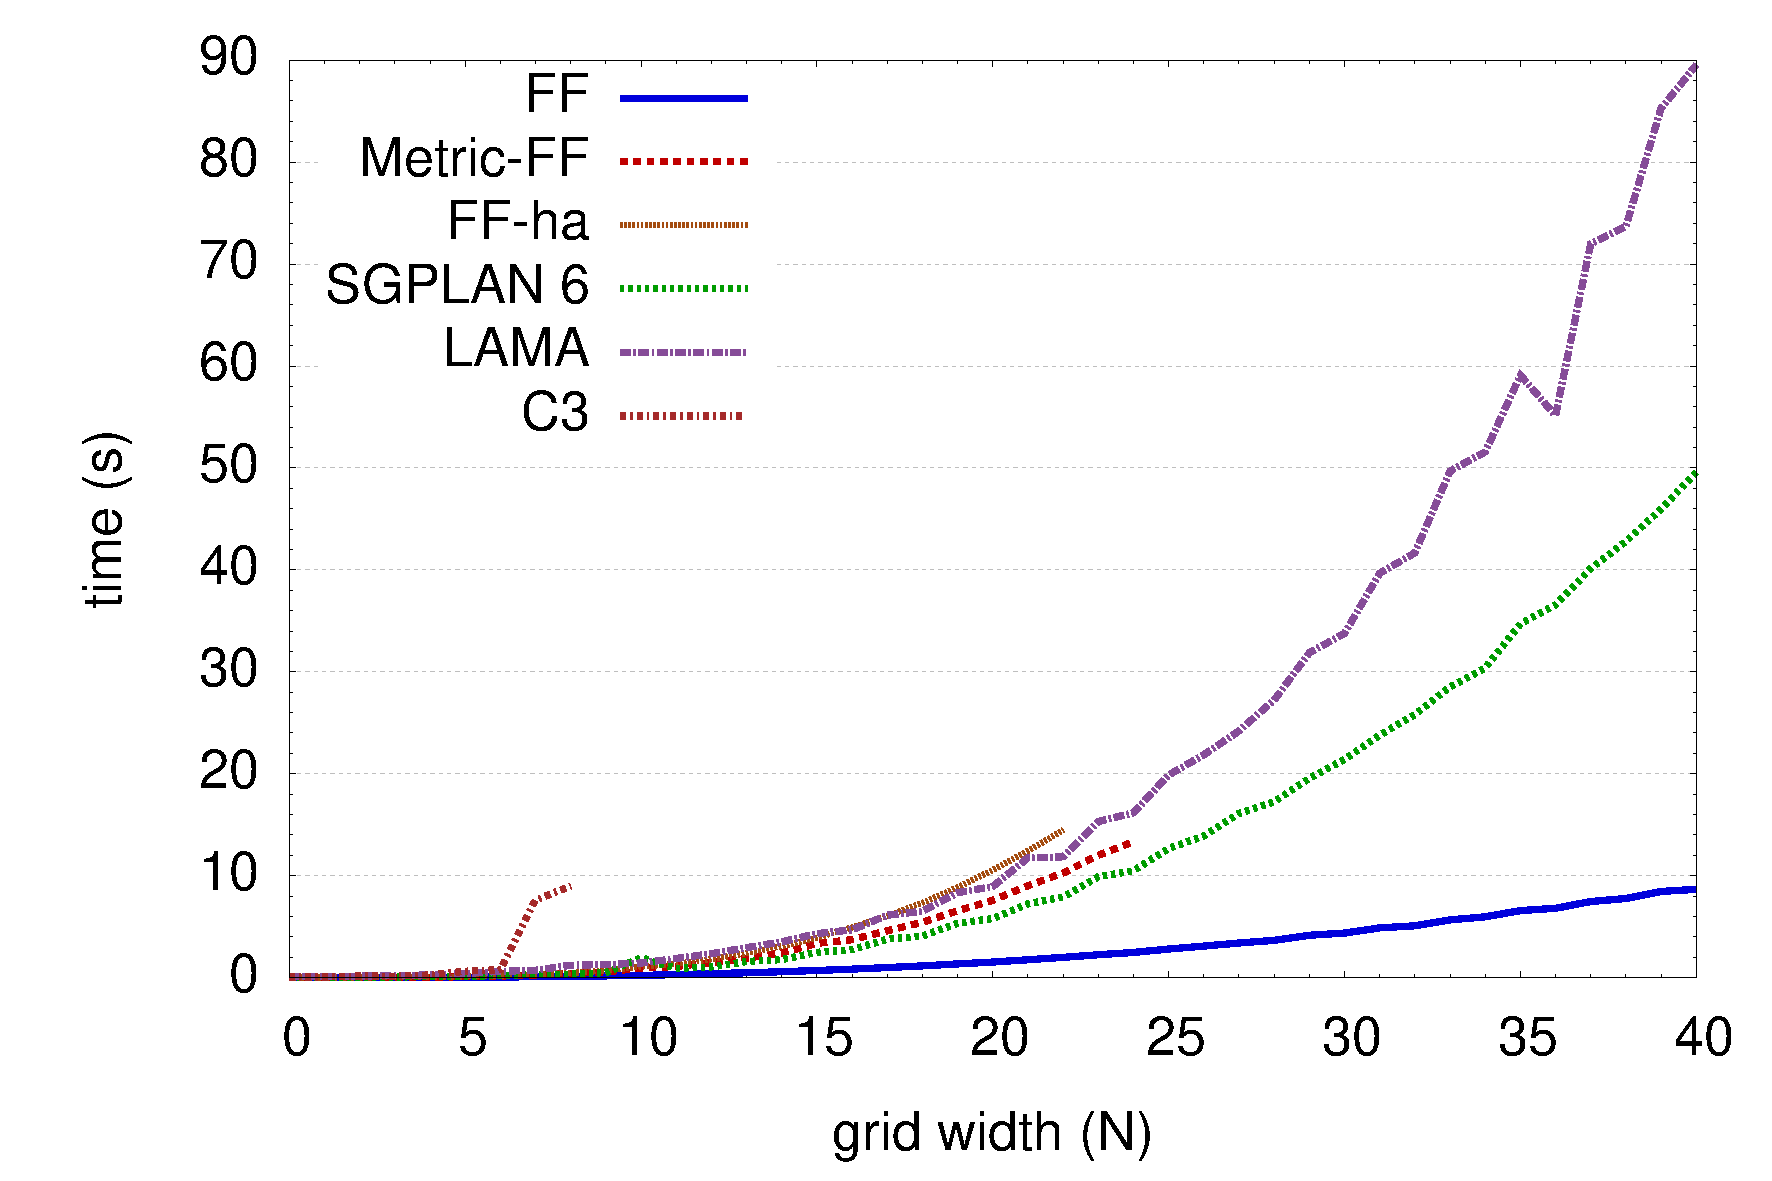
\includegraphics[width=7cm]{data/give2-minimal.pdf}}
  \caption{Results for the unordered and ordered minimal GIVE domains with grid
  height $h=20$. The horizontal axis is the grid width, $N$. 
  The vertical axis is the total runtime in seconds.}
  \label{fig:give-minimal}
\end{figure}

Results for the $h=20$ case, with the grid width $N$ ranging from $1$ to $40$,
are shown in Figure~\ref{fig:give-minimal}. In the unordered case
(Figure~\ref{fig:give-minimal}(a)), the most obvious result is that some of the
planners tested---Metric-FF, FF(h$_a$), and C$^3$---are unable to solve any
problems beyond $N=24$ on our experimentation machine within the memory limit of
2 GB.\footnote{All runtimes in Sections~\ref{sec:exper-3:-minim} and
 \ref{sec:experiment-4:-give} were measured on a single core of an Intel Xeon
 CPU running at 3GHz, under Linux. All runtimes are averaged over three runs of
 the planners. Only 32-bit versions of the planners were used for testing in
 each case.}
While FF, LAMA, and SGPLAN are able to solve all problem instances up to $N=40$,
the total running time varies greatly between these planners. For instance, FF
takes almost 35 seconds to solve the $N=40$ problem, while LAMA takes around 6.5
seconds. SGPLAN shows impressive performance on $N=40$, generating a 240 step
plan in well under a second. In the ordered case
(Figure~\ref{fig:give-minimal}(b)), we again have the situation where Metric-FF,
FF(h$_a$), and C$^3$ are unable to solve all problem instances. Furthermore,
both SGPLAN and LAMA, which performed well on the unordered problem, now perform
much worse than FF: FF takes 39 seconds for the $N=40$ case, while SGPLAN takes
50 seconds and LAMA takes 90 seconds. In real NLG systems, where response time
is essential, running times over a few seconds are unacceptable.

Preprocessing (parsing, grounding, etc.) time generally plays less of a role in
GIVE, compared with the sentence generation domain, however, its effects still
contribute significantly to the overall running time of a number of planners.
Figure~\ref{fig:give-minimal-grounding} shows the grounding time for FF, LAMA,
and SGPLAN on the minimal GIVE problems, compared with the total running time.
In the unordered variant of the minimal GIVE domain
(Figure~\ref{fig:give-minimal-grounding}(a)), the grounding time in LAMA and
SGPLAN accounts for a significant fraction of the total runtime: SGPLAN spends
around 40\% of its total runtime on preprocessing; for LAMA, this number
rises to at least 80\% for our test problems. For FF, the preprocessing time is
much less important than the search time, especially for large problem
instances. In the ordered case (Figure~\ref{fig:give-minimal-grounding}(b)), the
actual time spent on preprocessing is essentially unchanged from the unordered
case, and search time dominates the total runtime for all three planners.
Overall, however, FF is now much better at controlling the search, compared with
the other planners and its performance on the unordered variant of the problem.


\begin{figure}[t]
\subfloat[(a) Unordered]{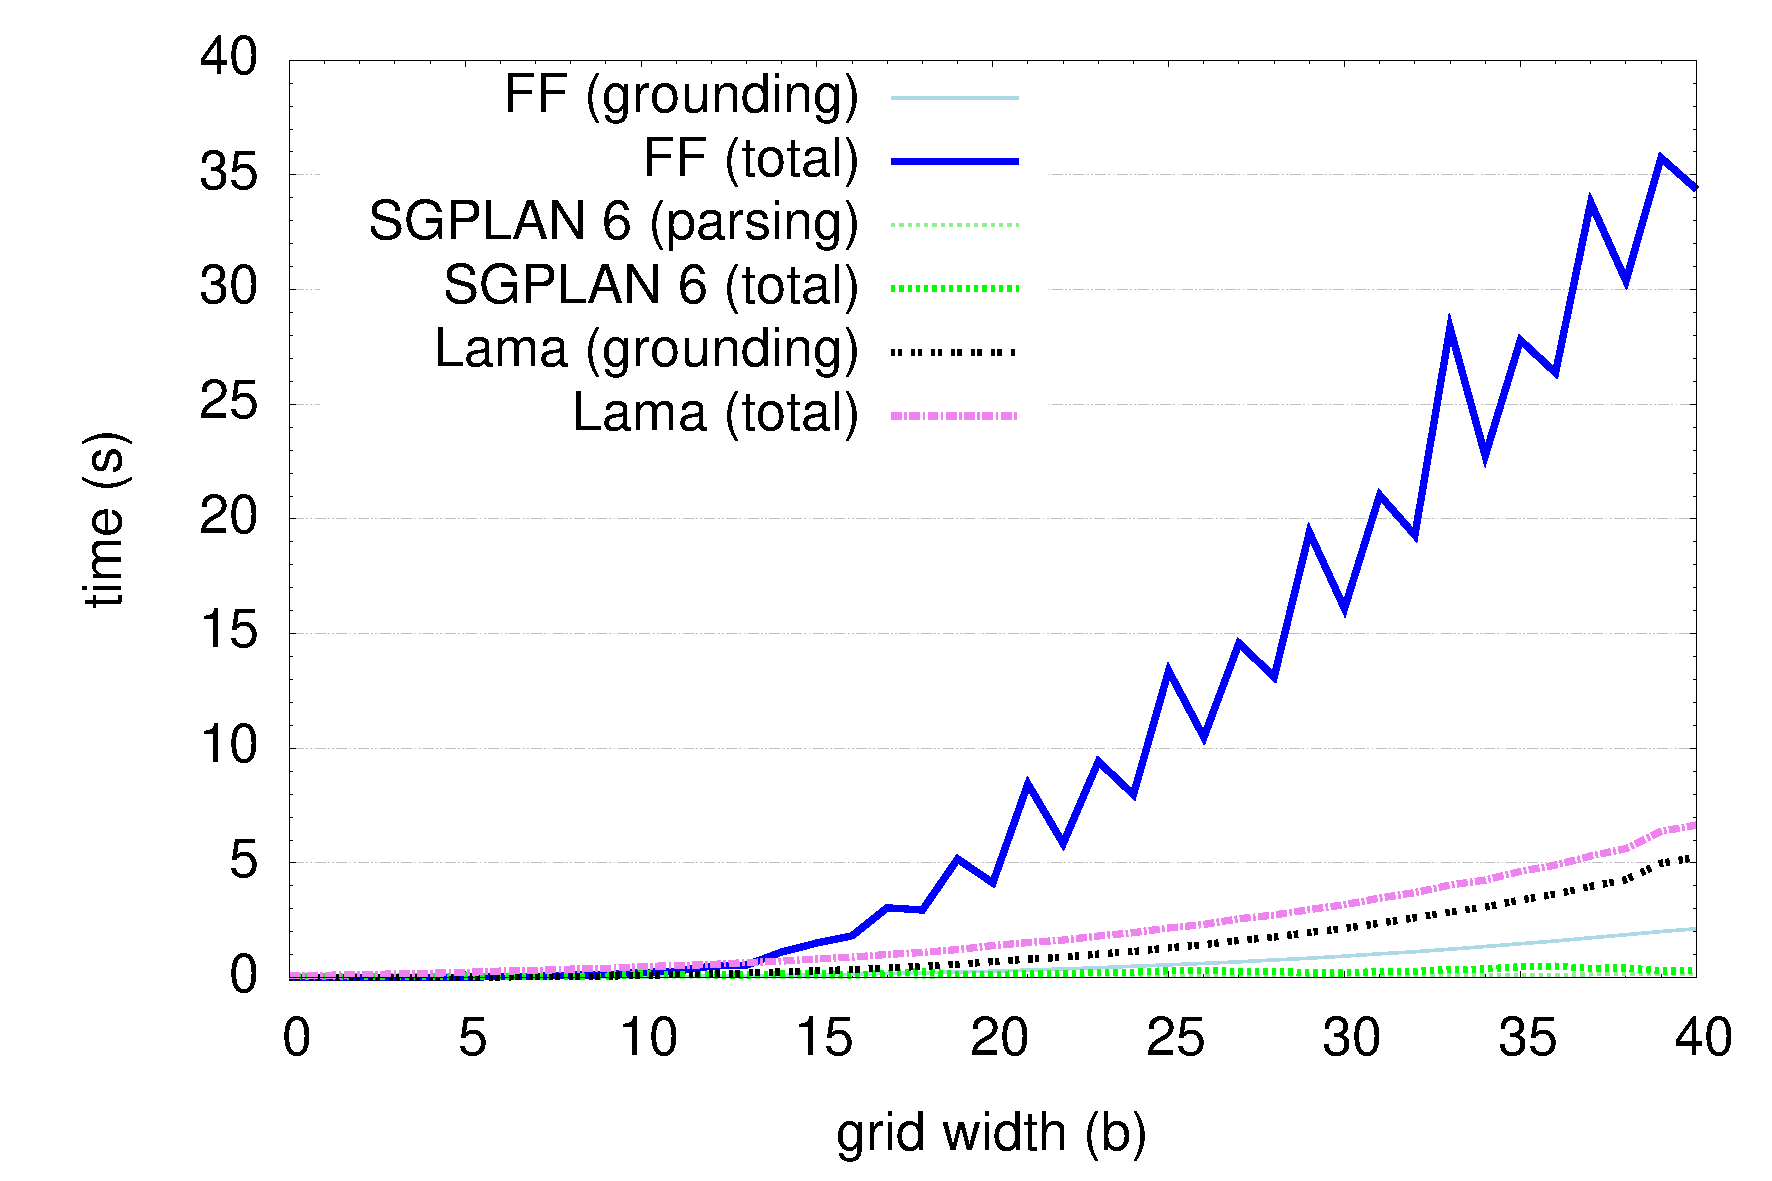
\includegraphics[width=7cm]{data/give-minimal-grounding.pdf}}
\subfloat[(b) Ordered]{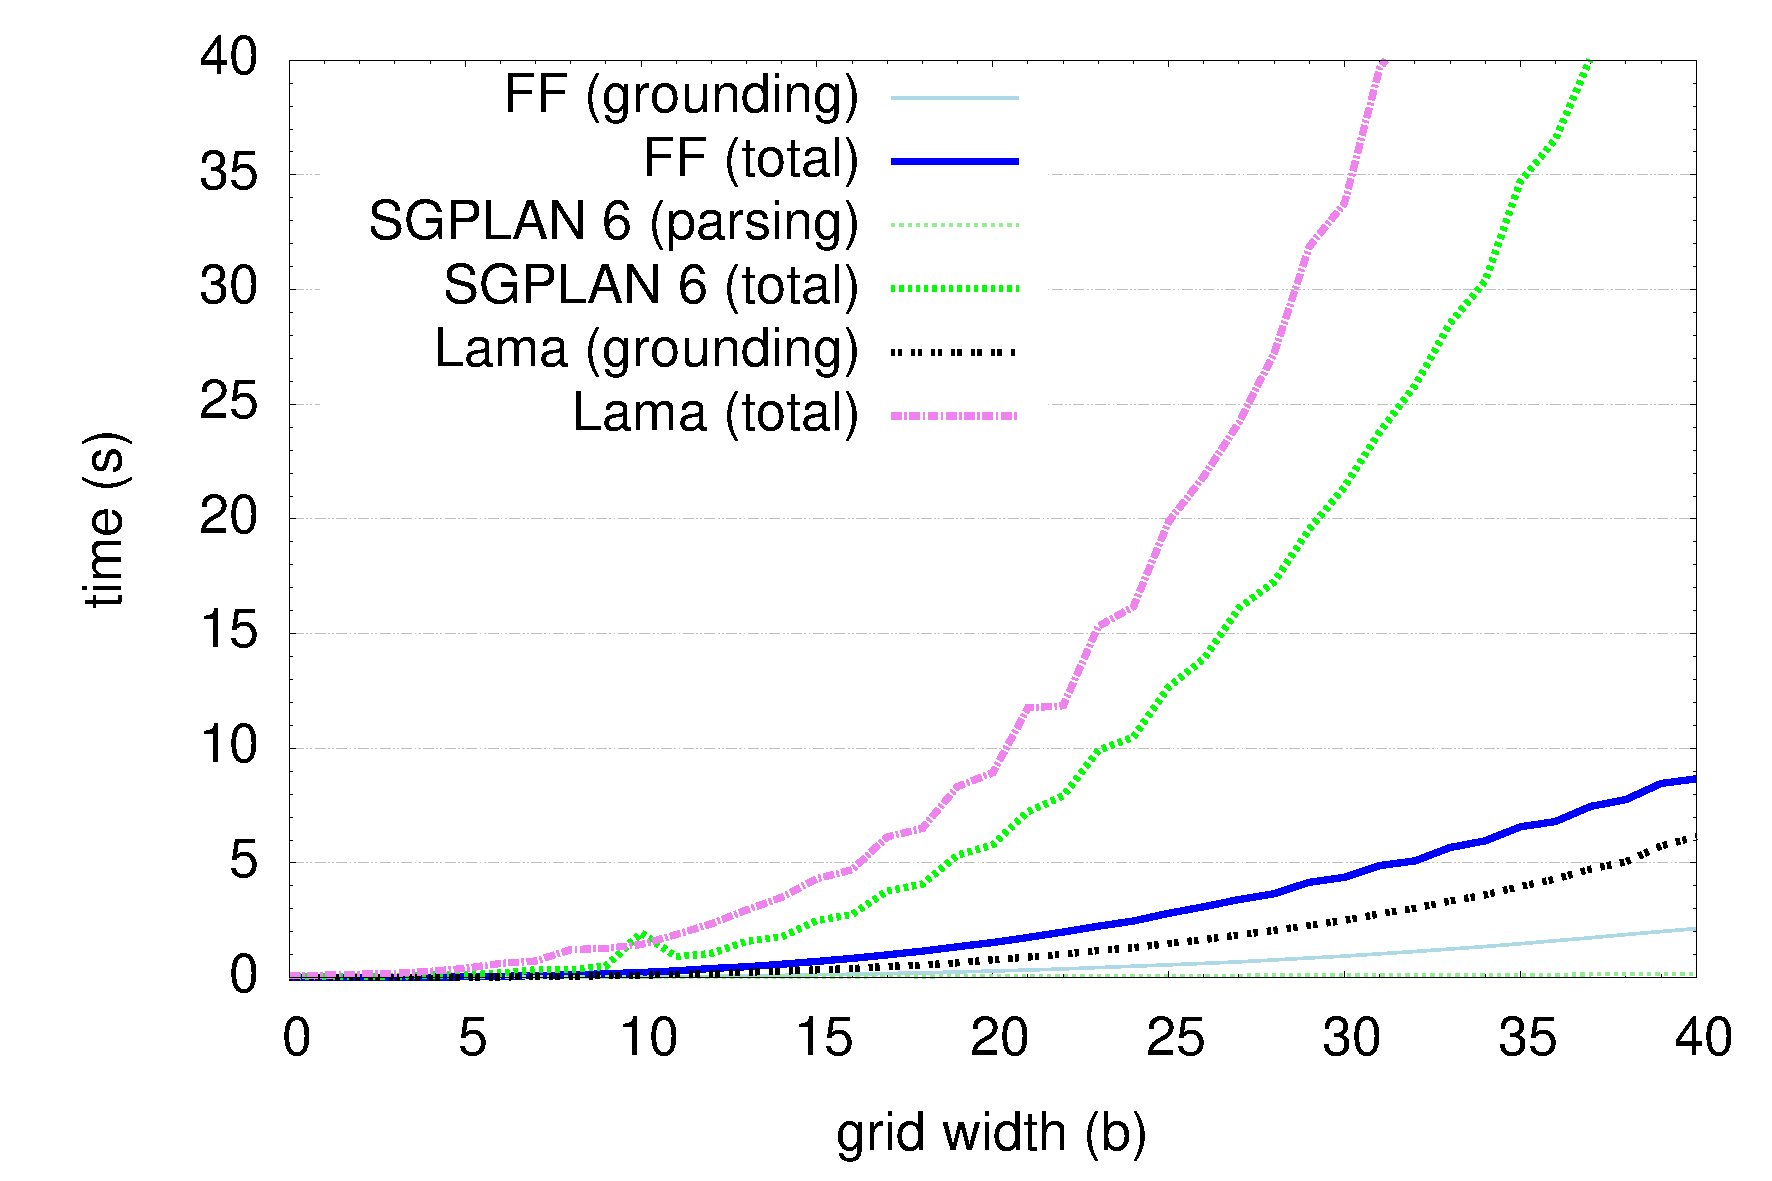
\includegraphics[width=7cm]{data/give2-minimal-grounding.pdf}}
  \caption{Comparison of the total running time and grounding time for selected
  planners in the $h=20$ minimal GIVE domain. The horizontal axis is the grid
  width, $N$. The vertical axis is the total runtime in seconds.}
  \label{fig:give-minimal-grounding}
\end{figure}



\subsection{Experiment 4: GIVE worlds with extra grid cells}
\label{sec:experiment-4:-give}

In our last set of experiments, we vary the structure of the GIVE world in order
to judge the effect that universe size has on the resulting planning problem.
Starting with the GIVE world described in Experiment~3, we extend the world map
by adding another $w$ by $h$ empty cell positions to the right of the minimal
world, as shown in Figure~\ref{fig:give-maps}(b). These new positions are not
actually required in any plan, but extend the size of the state space and
approximate the situation in the actual GIVE domain where most grid positions
are never used. We leave the initial state and goal untouched and, again,
consider both unordered and ordered variants of the problem.

Results for the $h=20$, $n=10$ case with $w$ ranging from $1$ to $40$ are shown
in Figure~\ref{fig:give-extracells}. As in Experiment~3, a number of planners
again fail to solve all the problems: Metric-FF, FF(h$_a$), and C$^3$ solve only
a few instances, while FF only scales to $w=23$. In the unordered version of the
domain, SGPLAN easily solves inputs beyond $w=40$ in well less than a second.
LAMA is also reasonably successful on these problems, however, its runtimes grow
more quickly than SGPLAN, with LAMA taking almost 5 seconds to solve the $w=40$
problem instance. In the ordered case, we again see behaviour similar to that of
Experiment~3: for the problem instances FF is able to solve, it performs
significantly better than LAMA and SGPLAN. (SGPLAN's long term runtime
appears to be growing at a slower rate than FF's, and so even if FF could be
scaled to larger problem instances, it seems possible that SGPLAN might overtake
FF as the better performer.) However, the overall planning times for most of
these instances are concerning since times over a couple seconds will negatively
affect the response time of an NLG system, which must react in real time to user
actions.

Finally, we also performed a set of experiments designed to investigate the
tradeoff between grounding time and search time on certain grid configurations.
For these experiments, we initially fixed the size of the grid and then varied
the number of buttons $b$ in the world, thereby creating a series of
``snapshots'' of particular extra-cell GIVE domains.
Figure~\ref{fig:give-buttons} shows the results of these experiments for the FF
and SGPLAN planners, for a fixed size grid of height 20 and width 40, and the
number of buttons $b$ ranging from 1 to 40. In each case, the amount of time a
planner spends on grounding is relatively unchanged as we vary the number of
buttons in a grid, while the search time continues to rise (sometimes quite
dramatically), as $b$ increases (we saw a similar effect for other grid
configurations we tried). This observation has important consequences for the
design of our GRID worlds: changing the underlying domain structure, even
minimally, may result in significant---and often unexpected---performance
differences for the planners that must operate in these domains.



\begin{figure}[t]
\subfloat[(a) Unordered]{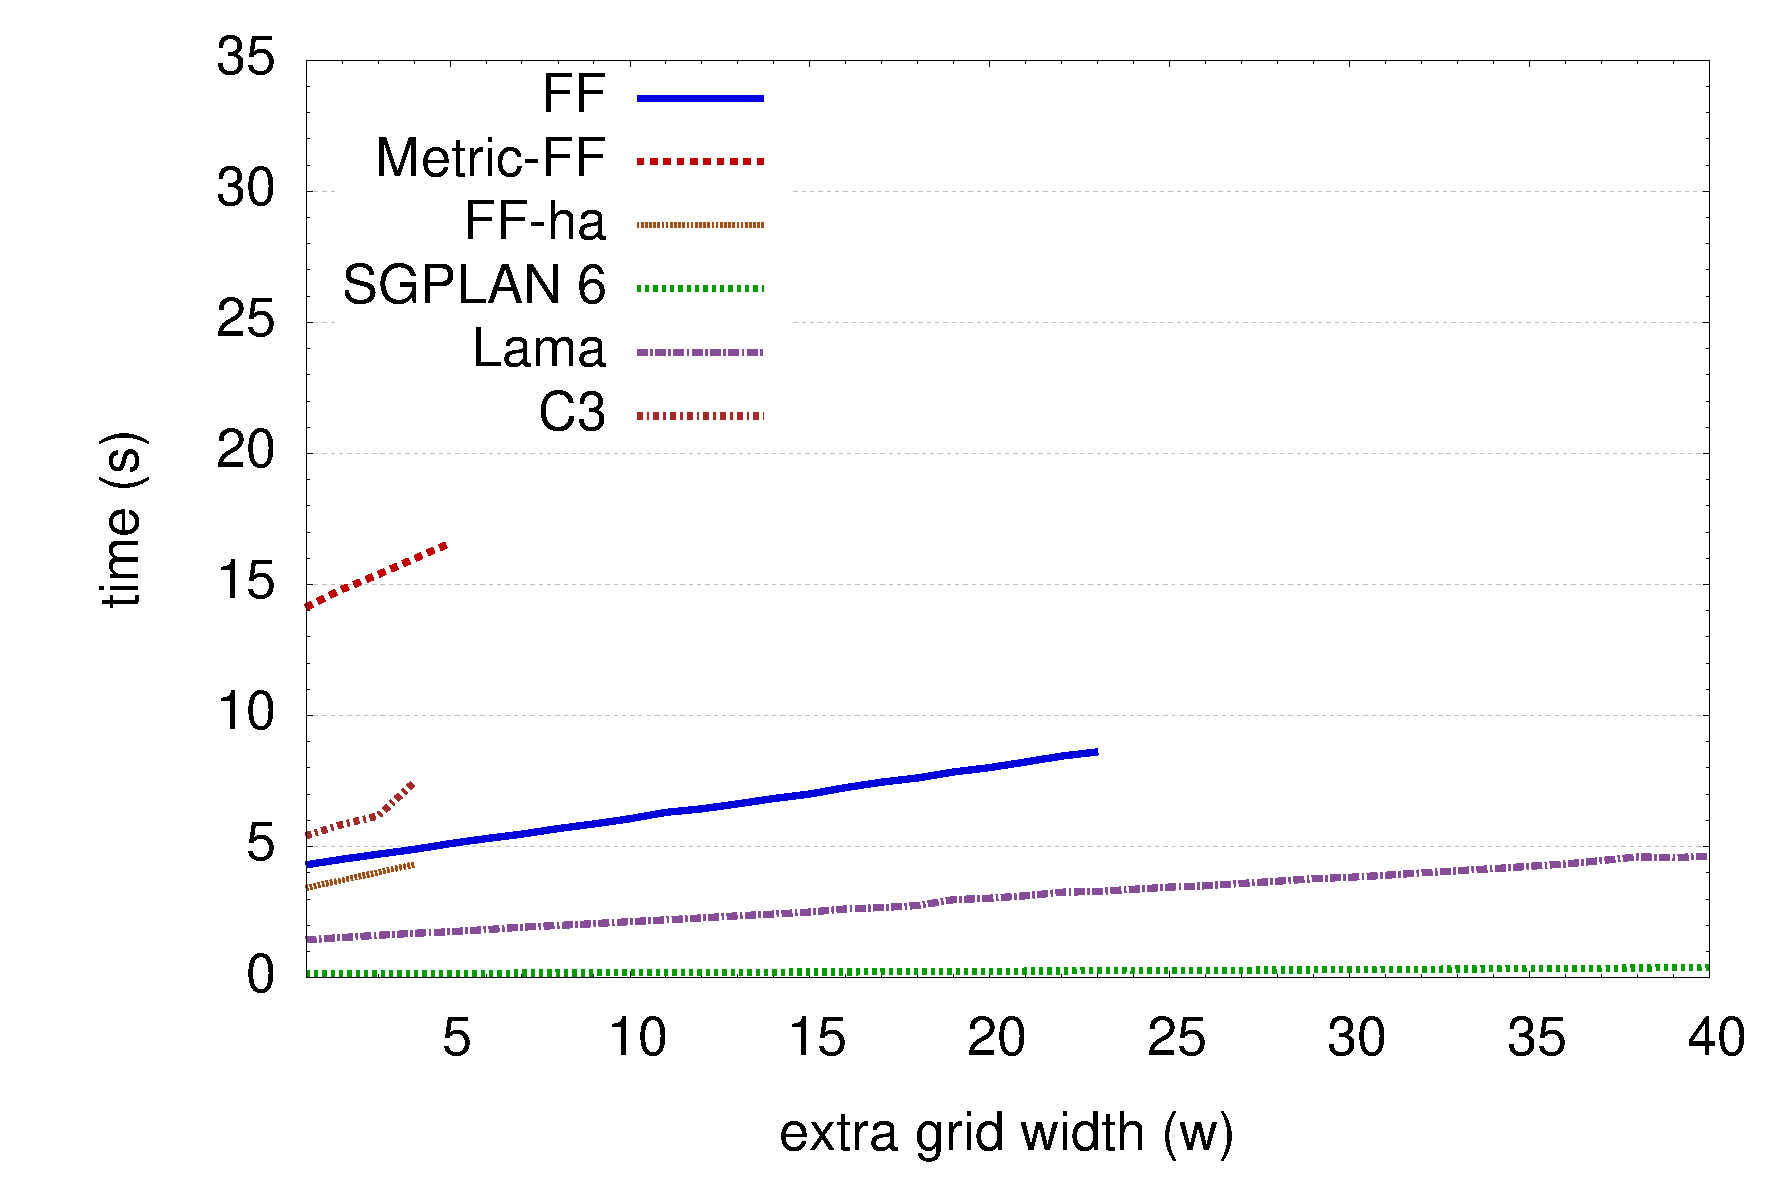
\includegraphics[width=7cm]{data/give-extracells.pdf}}
\subfloat[(b) Ordered]{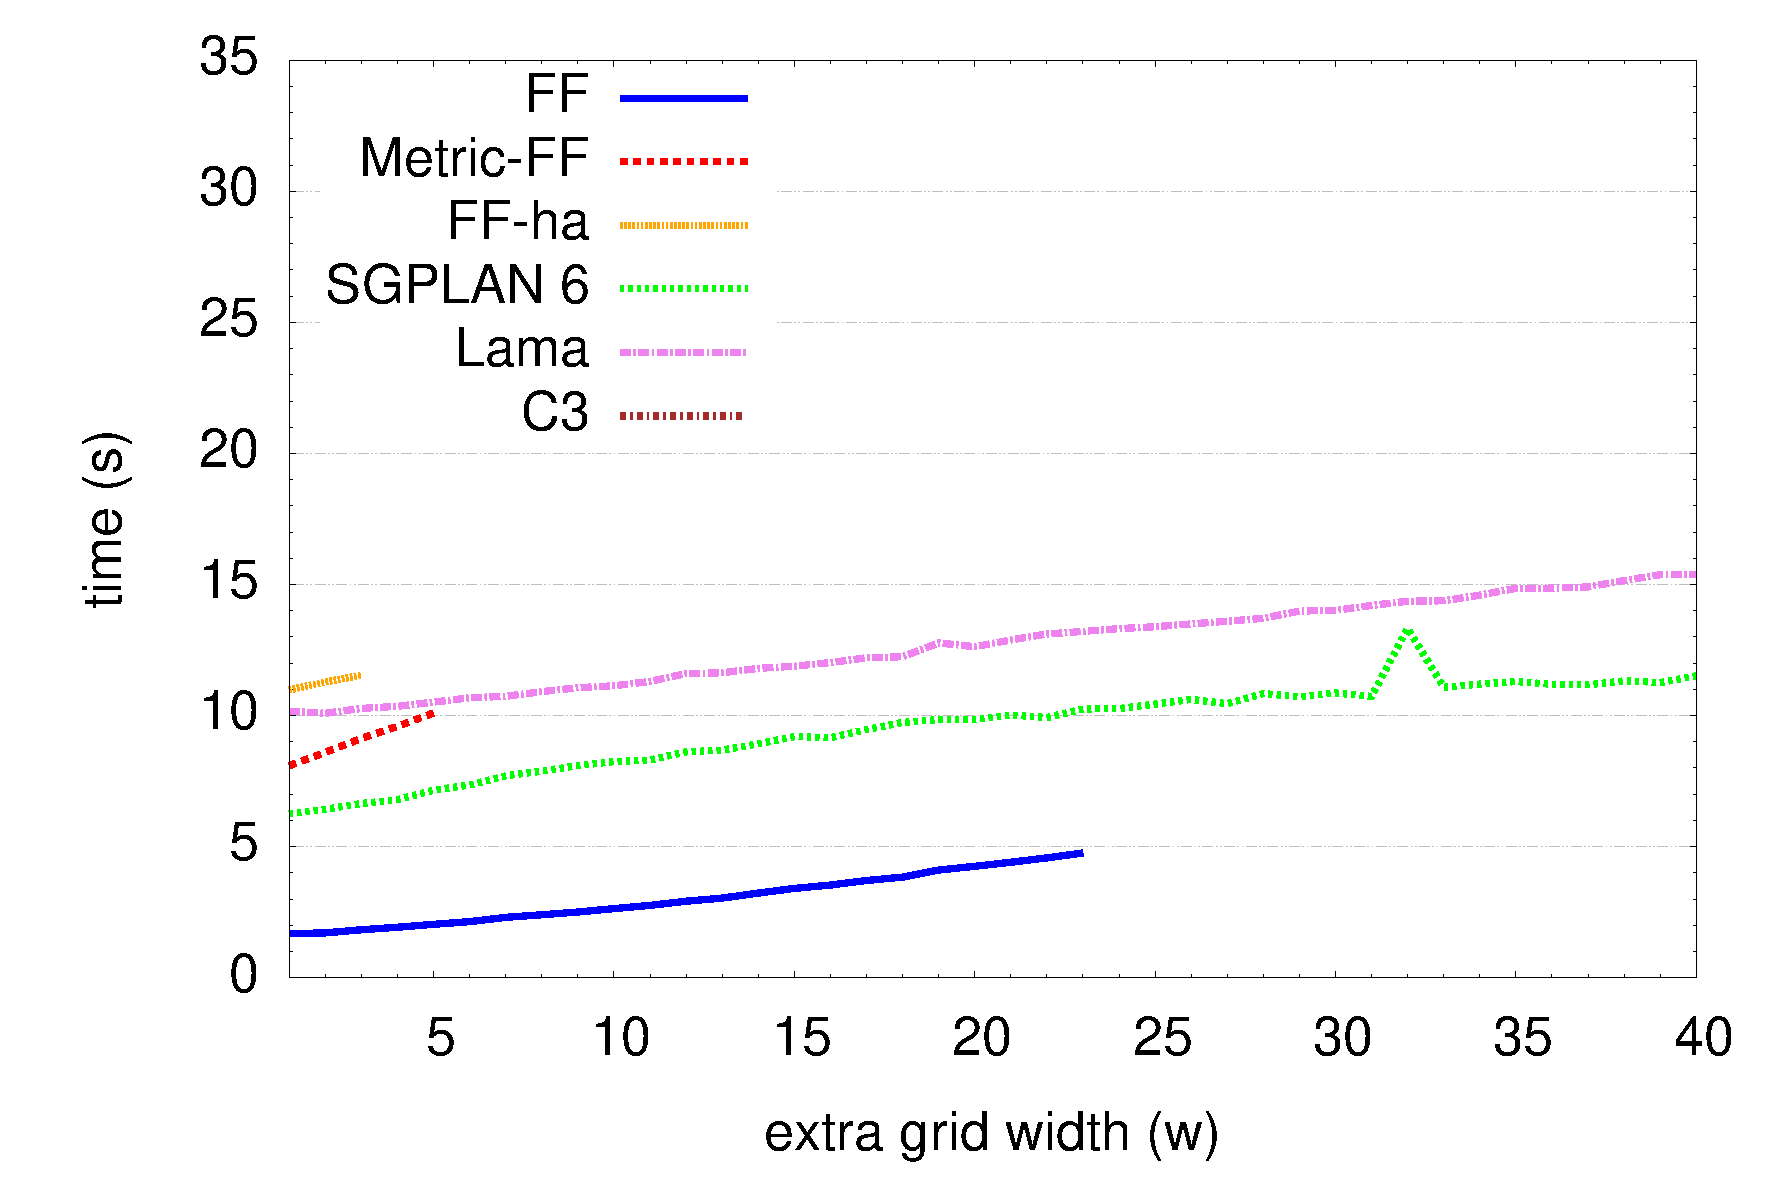
\includegraphics[width=7cm]{data/give2-extracells.pdf}}
  \caption{Results for the unordered and ordered GIVE domains with $h = 20$ and
  $n = 10$. The horizontal axis is the extra grid width $w$.
  The vertical axis is the total runtime in seconds.}
  \label{fig:give-extracells}
\end{figure}


\begin{figure}[t]
\subfloat[(a) Unordered]{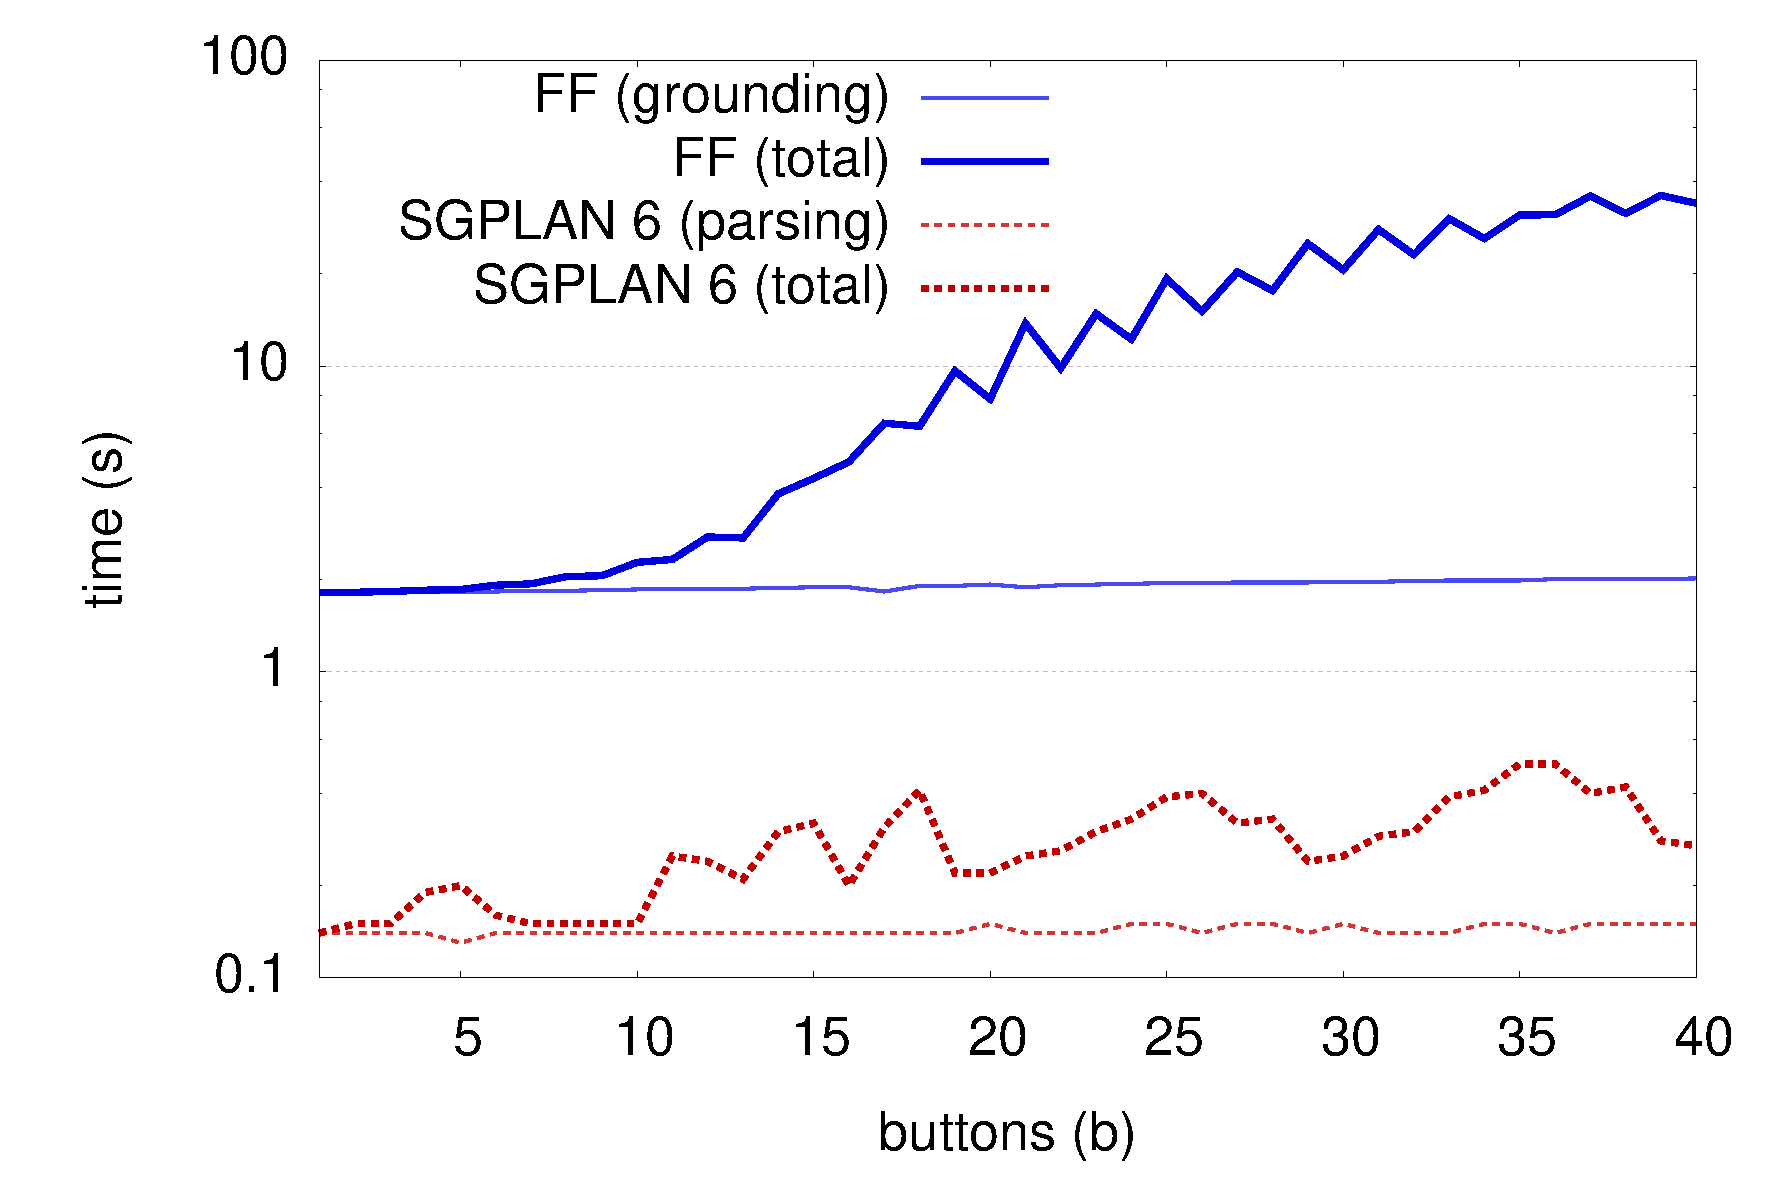
\includegraphics[width=7cm]{data/give-button-unord.pdf}}
\subfloat[(b) Ordered]{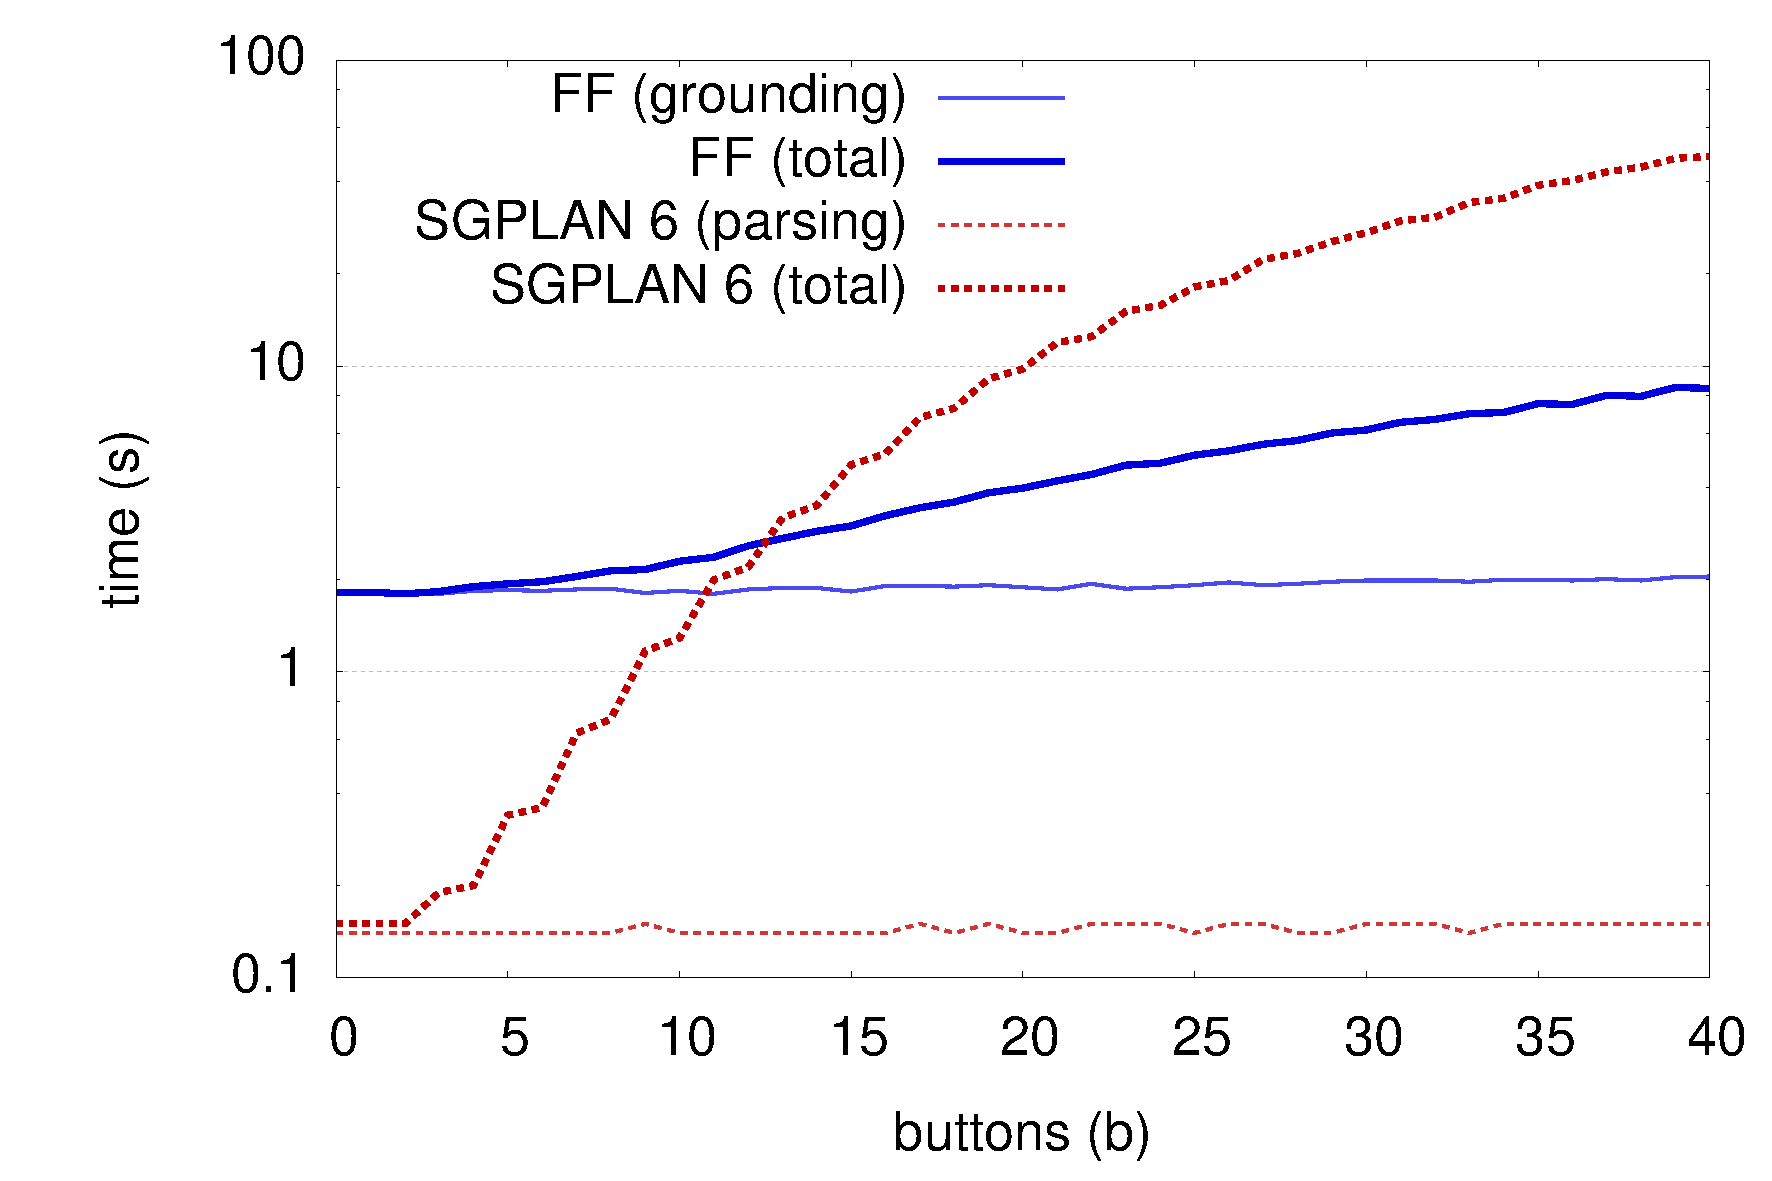
\includegraphics[width=7cm]{data/give-button-ord.pdf}}
  \caption{Results for the GIVE domains with a fixed grid size of
  height 20 and width 40. The horizontal axis is the number of buttons $b$.
  The vertical axis is the runtime in seconds (log scale).}
  \label{fig:give-buttons}
\end{figure}


%In the final experiment, we consider a variation on the GIVE worlds from
%Experiment~3. As before, we begin with a base grid of $2n$ by $h$
%positions, with buttons at positions $(2i-1,1)$ and $(2i,h)$ for $1 \leq i
%\leq n$. We then generate a second grid of $w$ by $h$ positions and place
%an additional button in this grid. Unlike Experiment~3, the second grid
%does not extend the first grid but is ``disconnected'' so its positions are
%inaccessible from the first grid, as shown in
%Figure~\ref{fig:give-maps}(c). Since the geometry of the grid makes it
%impossible to construct a plan for pressing all the buttons in the world,
%we instead investigate the time it takes a planner to arrive at the
%conclusion that the problem cannot be solved.

%Results for the $h=20$, $n=5$ case with $w$ ranging from 1 to 50 are shown
%in Figure.\footnote{FF and SGPLAN do
% not display runtimes when they fail to construct a plan so an external timing
% program was used to generate these results.}
%In this case, the runtimes for FF rise sharply around $w=28$, producing
%times that are unacceptable for an NLG system in practice. FF is unable
%to complete problem instances above $w=35$. SGPLAN, by comparison, performs
%exceptionally well and is able to complete problems instances up to $w=50$
%in about 0.3 seconds and $w=80$ in about 0.6 seconds. These results
%demonstrate that SGPLAN has a significant advantage over FF in this
%experiment. 


%%% Local Variables: 
%%% mode: latex
%%% TeX-master: "manuscript"
%%% End: 
